\documentclass[11pt,a4paper]{article}
\usepackage[top=3cm, bottom=2cm, left=2cm, right=2cm]{geometry}
\usepackage[utf8]{inputenc}
\usepackage{amsmath, amsfonts, amssymb}
\usepackage{siunitx}
\usepackage[brazil]{babel}
\usepackage{graphicx}
\usepackage[margin=10pt,font={small, it},labelfont=bf, textfont=it]{caption}
\usepackage[dvipsnames, svgnames]{xcolor}
\DeclareCaptionFont{MediumOrchid}{\color[svgnames]{MediumOrchid}}
\usepackage[pdftex]{hyperref}
\usepackage{natbib}
\bibliographystyle{plainnat}
\bibpunct{\textcolor{MediumOrchid}{\textbf{[}}}{\textcolor{MediumOrchid}{\textbf{]}}}{,}{s}{}{}
\usepackage{color}
\usepackage{footnote}
\usepackage{setspace}
\usepackage{booktabs}
\usepackage{multirow}
\usepackage{subfigure}
\usepackage{fancyhdr}
\usepackage{leading}
\usepackage{indentfirst}
\usepackage{wrapfig}
\usepackage{mdframed}
\usepackage{etoolbox}
\usepackage[version=4]{mhchem}
\usepackage{enumitem}
\usepackage{caption}
\usepackage{titlesec}
\usepackage{tcolorbox}
\usepackage{tikz}
\usepackage{LobsterTwo}
\usepackage[T1]{fontenc}
\usepackage{fontspec}
\usepackage{txfonts}
\usepackage[bottom]{footmisc}
\tcbuselibrary{skins,breakable}
\sisetup{output-decimal-marker={.}}

\makeatletter
\def\footnoterule{\kern-3pt\color{MediumOrchid}\hrule\@width0.6\textwidth height 0.8pt\kern2.6pt}
\makeatother

\renewcommand{\footnotelayout}{\itshape\color{MediumOrchid}}

\AtBeginEnvironment{equation}{\fontsize{13}{16}\selectfont}


\titleformat{\section}{\LobsterTwo\huge\color{CarnationPink}}{\thesection.}{1em}{}
\titleformat{\subsection}{\LobsterTwo\huge\color{CarnationPink}}{\thesubsection}{1em}{}
\titleformat{\subsubsection}{\bf\LobsterTwo\Large\color{MediumOrchid}}{\thesubsubsection}{1em}{}


\DeclareCaptionLabelFormat{figuras}{\textcolor{DarkTurquoise}{Figura \arabic{figure}}}
\captionsetup[figure]{labelformat=figuras}

\makeatletter
\renewcommand\tagform@[1]{\maketag@@@{\color{CarnationPink}(#1)}}
\makeatother

\renewcommand{\theequation}{Eq. \arabic{equation}}
\renewcommand{\thefigure}{Fig. \arabic{figure}}
\renewcommand{\thesection}{\textcolor{CarnationPink}{\arabic{section}}}

\setlist[itemize]{label=\textcolor{CarnationPink}{$\blacksquare$}}

\setlist[enumerate]{label=\textcolor{CarnationPink}{\arabic*.}, align=left, leftmargin=1.5cm}


\newcounter{exemplo}

\NewDocumentEnvironment{exemplo}{ O{} }{%
\allowbreak
\setlength{\parindent}{0pt}
  \begin{mdframed}[
  leftline=true,
  topline=false,
  rightline=false,
  bottomline=false,
  linewidth=2pt,
  linecolor=CarnationPink,
  frametitlerule=false,
  frametitlefont=\LobsterTwo\large\color{CarnationPink},
  frametitle={\color{CarnationPink}\LobsterTwo\large #1},
  ]
}{%
  \end{mdframed}
}

\setlength{\fboxsep}{5pt}
\setlength{\fboxrule}{1.5pt}
\usepackage{float}
\renewcommand{\thefootnote}{\alph{footnote}}
\usepackage{url}
\hypersetup{
	colorlinks=true,
	linkcolor=DarkTurquoise,
	filecolor=DarkTurquoise,      
	urlcolor=DarkTurquoise,
	citecolor=DarkTurquoise,
	pdftitle={Especialista em Física da Radioterapia}
}
\pagestyle{fancy}
\fancyhf{}
\renewcommand{\headrulewidth}{0pt}
\rfoot{\color{DarkTurquoise}\thepage \\ \LobsterTwo{\small\textcolor{CarnationPink}{@defDalila}}}

\title{\LobsterTwo\Huge{Radioterapia}}
\author{\LobsterTwo\LARGE{Análise de Distribuição de Dose e Espalhamento\nocite{*}}}
\date{\LobsterTwo{Dalila Mendonça}}
\begin{document}
	\maketitle

\section{Introdução}

	Quando um feixe de fótons se propaga pelo ar ou pelo vácuo, seu comportamento é governado pela \textcolor{DarkTurquoise}{\textbf{\textit{lei do inverso do quadrado}}}, onde a \textcolor{MediumOrchid}{\textbf{\textit{intensidade do feixe diminui à medida que se afasta da fonte de radiação}}}. No entanto, quando o feixe de fótons passa através de um fantoma (objeto simulador) ou um paciente, ele é afetado por três efeitos principais: \textcolor{MediumOrchid}{\textbf{\textit{atenuação}}}, \textcolor{MediumOrchid}{\textbf{\textit{espalhamento}}} e a \textcolor{MediumOrchid}{\textbf{\textit{lei do inverso do quadrado}}}. Esses efeitos combinados tornam a determinação da deposição de dose em um fantoma ou paciente uma tarefa desafiadora.

	A \textcolor{DarkTurquoise}{\textbf{\textit{atenuação}}} refere-se à \textcolor{MediumOrchid}{\textbf{\textit{redução da intensidade do feixe de fótons à medida que eles interagem e são absorvidos pelo material do fantoma ou paciente}}}. A atenuação depende das características do material e da energia dos fótons. Quanto maior a energia dos fótons, menor é a atenuação. 
	
	O \textcolor{DarkTurquoise}{\textbf{\textit{espalhamento}}} ocorre quando os \textcolor{MediumOrchid}{\textbf{\textit{fótons sofrem desvios em sua trajetória ao interagir com o material do fantoma ou paciente}}}. Esses desvios podem ser causados por espalhamento Compton e espalhamento Rayleigh. O espalhamento afeta a \textcolor{MediumOrchid}{\textbf{\textit{distribuição espacial da dose}}}. A lei do inverso do quadrado ainda se aplica, mas agora com as contribuições da atenuação e do espalhamento, o que torna a relação entre a intensidade do feixe e a distância da fonte mais complexa.

	Medir diretamente a distribuição de dose dentro de um paciente é praticamente impossível devido à complexidade e inacessibilidade do interior do corpo humano. No entanto, é crucial ter um \textcolor{MediumOrchid}{\textbf{\textit{conhecimento preciso e exato da distribuição de dose dentro do volume irradiado}}} para garantir um tratamento por radiação bem-sucedido. Uma abordagem comum é \textcolor{MediumOrchid}{\textbf{\textit{estabelecer várias funções matemáticas}}} que relacionam a dose em qualquer ponto dentro do paciente com a dose conhecida em um ponto de calibração do feixe em um fantoma. 
	
	O \textcolor{DarkTurquoise}{\textbf{\textit{fantoma}}} é um objeto de referência que possui \textcolor{MediumOrchid}{\textbf{\textit{características semelhantes ao tecido humano}}} e é utilizado para \textcolor{MediumOrchid}{\textbf{\textit{calibrar}}} o sistema de medição. Ao medir a dose em pontos específicos do fantoma e relacioná-la às doses em pontos correspondentes dentro do paciente, é possível obter uma estimativa da distribuição de dose dentro do paciente.

	Essas \textcolor{MediumOrchid}{\textbf{\textit{funções}}} são geralmente determinadas utilizando \textcolor{MediumOrchid}{\textbf{\textit{detectores de radiação apropriados}}} colocados em \textcolor{MediumOrchid}{\textbf{\textit{fantomas}}} que têm características semelhantes ao tecido humano. Os detectores registram a \textcolor{MediumOrchid}{\textbf{\textit{dose ou taxa de dose}}} em pontos específicos do fantoma. A dose ou taxa de dose no \textcolor{MediumOrchid}{\textbf{\textit{ponto de referência}}}, que é o ponto de calibração do feixe, é determinada usando fantomas de água. Os fantomas de água são utilizados porque a água tem \textcolor{MediumOrchid}{\textbf{\textit{propriedades de atenuação semelhantes às do tecido humano}}}. A determinação da dose no ponto de referência é realizada em \textcolor{MediumOrchid}{\textbf{\textit{condições de referência específicas}}}, como profundidade, tamanho de campo e distância fonte-superfície (SSD), que são padronizadas e bem definidas.

	A \ref{fig:pdpSaida} ilustra uma distribuição típica de dose ao longo do eixo central de um feixe de fótons de alta energia incidente em um paciente. Diversos pontos e regiões importantes podem ser identificados nessa distribuição. O feixe de fótons entra no paciente na superfície, fornecendo uma \textcolor{MediumOrchid}{\textbf{\textit{dose superficial}}} específica ($D\text{s}$). À medida que o feixe penetra no paciente, a dose aumenta rapidamente inicialmente até atingir um \textcolor{MediumOrchid}{\textbf{\textit{valor máximo}}} em uma certa profundidade ($z_{max})$. Essa profundidade varia dependendo das características do feixe e do tipo de tratamento. Após atingir o valor máximo, a dose começa a \textcolor{MediumOrchid}{\textbf{\textit{diminuir quase exponencialmente}}} à medida que o feixe se propaga através do paciente. No ponto de saída do paciente, a dose atinge um valor específico ($D\text{ex}$), que é determinado pela interação do feixe com os tecidos e a geometria do tratamento.

	\begin{figure}[h]
		\centering
		\fcolorbox{DarkTurquoise}{white}{%
			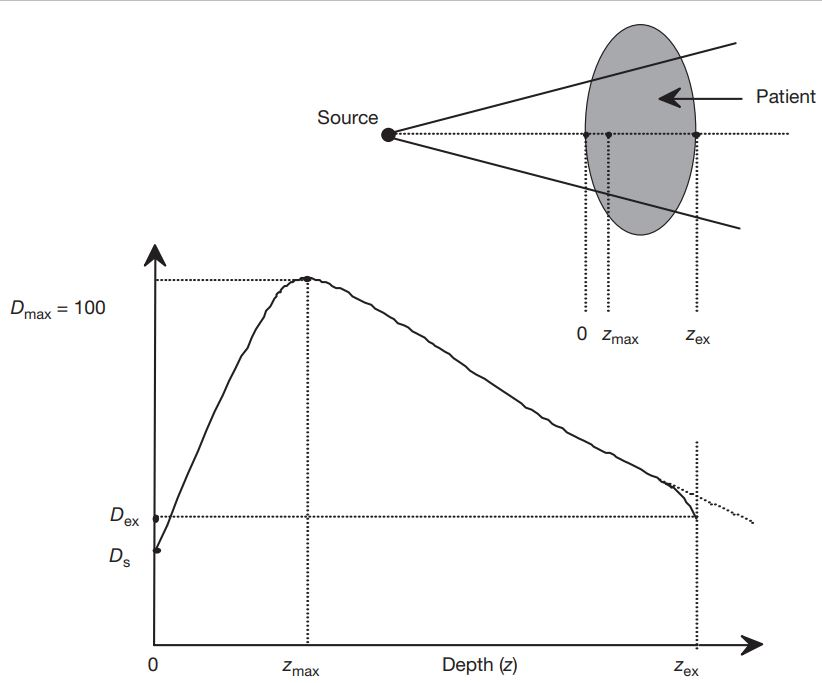
\includegraphics[width=0.5\textwidth]{Imagens/pdpSaida.JPG
			}
		}%
		\caption{Deposição de dose de um feixe de fótons de megavoltagem em um paciente. Ds é a dose de superfície no lado de entrada do feixe, Dex é a dose de superfície no lado de saída do feixe. Dmax é a dose máxima geralmente normalizada para 100, resultando em uma curva de dose em profundidade conhecida como distribuição de dose em profundidade percentual (PDD). A região entre z = 0 e z = zmax é referida como a região de acúmulo de dose.}
		\label{fig:pdpSaida}
	\end{figure}

	A \textcolor{MediumOrchid}{\textbf{\textit{dose de saída}}} se refere à quantidade de dose que é entregue ao paciente no ponto de saída do feixe de radiação. Na \ref{fig:pdpSaida}, é possível observar que, próximo ao ponto de saída do feixe, \textcolor{MediumOrchid}{\textbf{\textit{as curvas de distribuição de dose apresentam uma ligeira inclinação para baixo}}} em relação à curva de distribuição de dose extrapolada. Isso significa que a dose medida nessa região é ligeiramente menor do que o valor esperado. Essa pequena divergência ocorre devido à falta de contribuição de espalhamento proveniente de áreas além do ponto de saída. No ponto de saída, as áreas além desse ponto não contribuem significativamente para a dose medida devido ao espalhamento limitado no meio de ar.

\section{Phantoms}

	Normalmente são feitos de \textcolor{MediumOrchid}{\textbf{\textit{água ou material água-equivalente}}} para manter as mesmas características de absorção e espalhamento dos músculos e outros tecidos moles.

	Um \textcolor{DarkTurquoise}{\textbf{\textit{material água equivalent}}}e para feixes de megavoltagem devem possuir a mesma densidade eletrônica da água, que é o parâmetro relacionado à probabilidade de interação nas faixas de energia onde predomina o efeito Compton. A densidade eletrônica de um meio é dada pela \ref{eq:densidadeEletronica}:

		\begin{equation}
			\rho_e = \rho_m \cdot N_A \cdot \left(\frac{Z}{A}\right)
			\label{eq:densidadeEletronica}
		\end{equation}

		\begin{exemplo}[onde:]
			\begin{itemize}
				\begin{equation}
							\frac{Z}{A} = \sum_{i} a_i \cdot \frac{Z_i}{A_i}
				\end{equation}
				\item \textcolor{DarkTurquoise}{$\mathbf{\rho_m}$} é a densidade mássica do meio;
				\item \textcolor{DarkTurquoise}{$\mathbf{N_A}$} é o número de Avogadro;
				\item \textcolor{DarkTurquoise}{$\mathbf{a_i}$} é a fração de peso do i-ésimo elemento que constitui a molécula;
				\item \textcolor{DarkTurquoise}{$\mathbf{Z_i}$} é o número atômico do i-ésimo elemento;
				\item \textcolor{DarkTurquoise}{$\mathbf{A_i}$} é o número de massa do i-ésimo elemento.
			  \end{itemize}
		\end{exemplo}

	A \ref{fig:densidadeEletronica} mostra a densidade eletrônica dos principais tecidos de interesse dosimétrico, incluindo tecidos que compõem o corpo e a \ref{fig:materiaisPhanton} apresenta as propriedades físicas dos principais materiais dos phantoms utilizados.

		\begin{figure}[h]
			\centering
			\fcolorbox{DarkTurquoise}{white}{
			
				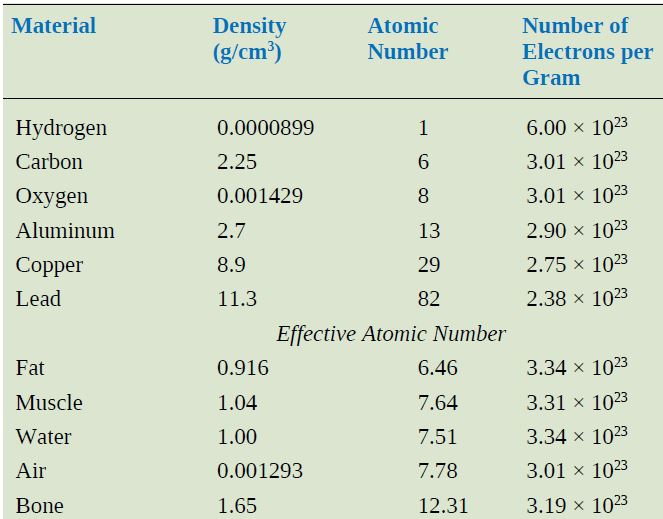
\includegraphics[width=0.5\textwidth]{Imagens/densidadeEletronica.JPG}
			}
			\caption{Densidade eletrônica de alguns tecidos de interesse}
			\label{fig:densidadeEletronica}
		\end{figure}

		\begin{figure}[h]
			\centering
			\fcolorbox{DarkTurquoise}{white}{%
			 	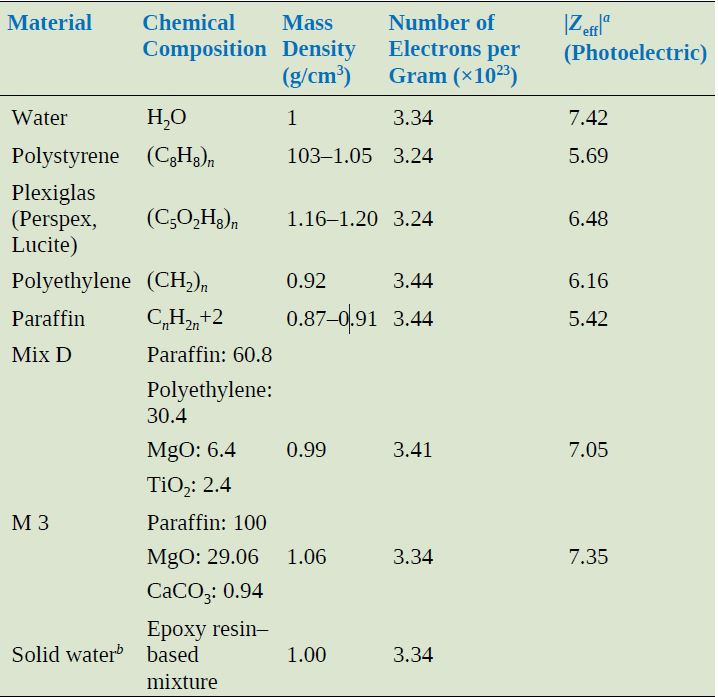
\includegraphics[width=0.5\textwidth]{Imagens/materiaisPhanton.JPG}
			}%
			\caption{Propriedades físicas de alguns materiais utilizados nos phantoms.}
			\label{fig:materiaisPhanton}
		\end{figure}


		\textcolor{DarkTurquoise}{\textbf{\textit{Phantoms antropomórficos}}} são aqueles que \textcolor{MediumOrchid}{\textbf{\textit{simulam o corpo humano}}} tendo a forma de um dorso e é composto por materiais que simulam diferentes tecidos como músculo, pulmão, osso e cavidades de ar. Esse phantom é dividido em diversas sessões (vários recortes) sendo possível inserir detectores de radiação como filmes, etc\dots


\section{Distribuição de Dose Na Profundidade}

	A dose absorvida em um meio varia com a profundidade e depende de vários fatores como: \textcolor{MediumOrchid}{\textbf{\textit{Energia do Feixe, profundidade, tamanho de campo, distância até a fonte e sistema de colimação do feixe}}}. O Primeiro passo é definir a variação da dose com a profundidade ao longo do eixo central do feixe e as outras quantidades de interesse são derivadas a partir dessa quantidade. As principais quantidades que determinam essa variação são : PDP, TAR, TPR e TMR. Normalmente essas quantidades são obtidas através de medidas com câmaras de ionização com pequenas cavidades. 

\subsection*{Porcentagem de Dose na Profundidade (PDP)}

	A \textcolor{DarkTurquoise}{\textbf{\textit{PDP}}} \textcolor{MediumOrchid}{\textbf{\textit{normaliza a dose na profundidade $d$ com respeito a dose na profundidade de referência ($d_0$)}}}, que para feixes de MV normalmente é definida na profundidade de dose máxima ($d_0 = d_{max}$) e para feixes de baixa energia é definido na superfície. A \ref{fig:pdp} mostra a geometria para a definição da PDP.

		\begin{figure}[h]
			\centering
			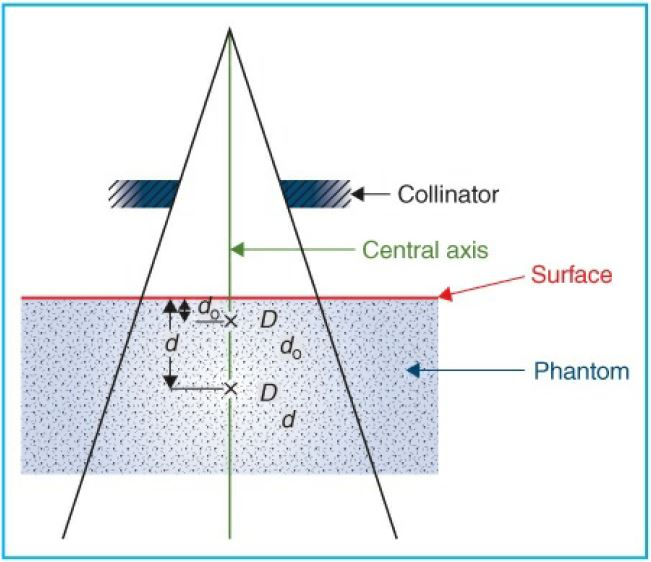
\includegraphics[width=0.5\textwidth]{Imagens/pdp.JPG}
			\caption{Porcentagem de Dose na Profundidade}
			\label{fig:pdp}
		\end{figure}

	A PDP é dada então pela seguinte equação:

		\begin{equation}
			PDP(d) = \frac{D_d}{D_{d_0}} \times 100 \%
		\end{equation}

	
	A profundidade de dose máxima para feixes de MV ocorrem em maiores profundidades dependendo da \textcolor{MediumOrchid}{\textbf{\textit{energia do feixe}}}, e também varia com o \textcolor{MediumOrchid}{\textbf{\textit{tamanho de campo}}}, uma vez que as variações no tamanho de campo alteram a \textcolor{MediumOrchid}{\textbf{\textit{quantidade de contaminação com elétrons}}} que atingem a superfície. Portanto $d_{max}$ deve ser determinado para um campo pequeno ($3 \times 3 \; cm^2$) para minimizar a contaminação com elétrons, e então se manterá a mesma para todos os tamanhos de campo independente de qual é a real profundidade onde o pico de dose ocorre. A PDP depende de alguns fatores como a \textcolor{MediumOrchid}{\textbf{\textit{energia do feixe}}} (qualidade do feixe), \textcolor{MediumOrchid}{\textbf{\textit{profundidade}}}, \textcolor{MediumOrchid}{\textbf{\textit{tamanho de campo e sua forma}}}, \textcolor{MediumOrchid}{\textbf{\textit{SSD}}} e \textcolor{MediumOrchid}{\textbf{\textit{colimação do feixe}}}. 

\subsubsection*{Dependência com a Qualidade Do Feixe E Profundidade}

		
	Além de $d_{max}$ \textcolor{MediumOrchid}{\textbf{\textit{a PDP diminui com a profundidade e aumenta com a energia do feixe}}}. Feixes de maiores energias são mais \textcolor{MediumOrchid}{\textbf{\textit{penetrantes}}} e portanto entregam uma maior PDP na profundidade. Ignorando os efeitos do Inverso do Quadrado da Distância (IQD), a PDP é governada aproximadamente pela atenuação exponencial de modo que a PDP é afetada pela qualidade do feixe através do coeficiente de atenuação médio $\bar{\mu}$. A medida que $\bar{\mu}$ diminui, o feixe é mais penetrante resultando em uma maior PDP em uma dada profundidade após a região de builup. 

	\begin{wrapfigure}{l}{0.5\textwidth}
		\centering
		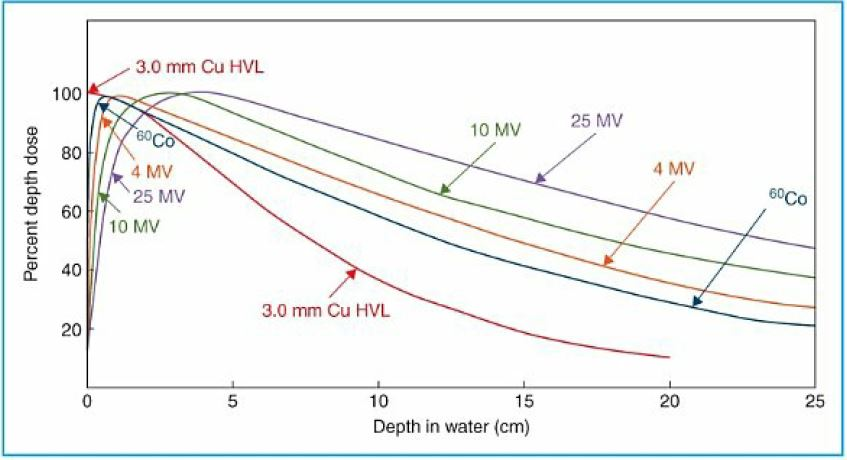
\includegraphics[width=0.48\textwidth]{Imagens/buildupDiferentesFeixes.JPG}
		\caption{Buildup para diferentes qualidades de feixe}
		\label{fig:buildupDiferentesFeixes}
	\end{wrapfigure}


	A \ref{fig:buildupDiferentesFeixes} mostra que a \textcolor{MediumOrchid}{\textbf{\textit{PDP diminui além da profundidade de dose máxima}}} e que o \textcolor{MediumOrchid}{\textbf{\textit{buildup de dose }}}(região entre a superfície e o ponto de profundidade de dose máxima) \textcolor{MediumOrchid}{\textbf{\textit{é maior com o aumento da energia}}}, onde a dose máxima ocorre aproximadamente na superfície para a qualidade com HVL de 3.0 mm Cu e em uma profundidade de $\sim 4$ cm para o feixe de fótons de 25 MV.

	Esse buildup de dose para feixes MV faz com que a dose na pele seja muito menor quando comparado à dose máxima, sendo chamado de \textcolor{MediumOrchid}{\textbf{\textit{efeito poupador da pele}}}; Porém é importante reforçar que possui uma menor dose relativa, o que nem sempre implica em uma dose baixa.		

	A medida que os \textcolor{MediumOrchid}{\textbf{\textit{fótons incidem no meio}}} (superfície do phantom ou do paciente), \textcolor{MediumOrchid}{\textbf{\textit{elétrons de alta energia}}} (rápidos) são liberados da superfície e das camadas subsequentes. Estes elétrons depositam sua energia até serem \textcolor{MediumOrchid}{\textbf{\textit{completamente parados no meio}}}, o que ocorre em uma distância significante abaixo de onde foram liberados; Por isso a \textcolor{MediumOrchid}{\textbf{\textit{fluência dos elétrons}}} e, portanto, a \textcolor{MediumOrchid}{\textbf{\textit{dose absorvida aumenta com a profundidade}}} até alcançar um máximo. No entanto, a \textcolor{MediumOrchid}{\textbf{\textit{fluência de fótons diminui continuamente com a profundidade}}} (uma vez que ao interagir com os elétrons, esse fóton é espalhado e deixa de fazer parte do feixe primário), e como resultado, \textcolor{MediumOrchid}{\textbf{\textit{a produção de elétrons também diminui com a profundidade}}}, de modo que o efeito líquido após uma certa profundidade é uma diminuição de dose absorvida. 

		\begin{wrapfigure}{r}{0.5\textwidth}
			\centering
			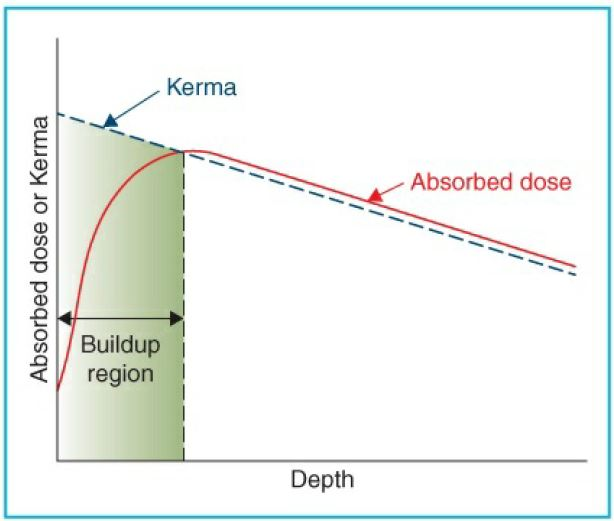
\includegraphics[width=0.48\textwidth]{Imagens/esquemaBuildup.JPG}
			\caption{Esquema do Buildup de Dose absorvida}
			\label{fig:esquemaBuildup}
		\end{wrapfigure}

	Como o \textcolor{DarkTurquoise}{\textbf{\textit{kerma}}} representa a \textcolor{MediumOrchid}{\textbf{\textit{energia transferida pelos fótons para partículas diretamente ionizantes}}} (elétrons), o kerma é \textcolor{MediumOrchid}{\textbf{\textit{máximo}}} na superfície e \textcolor{MediumOrchid}{\textbf{\textit{diminui com a profundidade}}} devido à diminuição da fluência de energia do feixe de fótons. Por outro lado, a \textcolor{MediumOrchid}{\textbf{\textit{dose absorvida}}} primeiramente \textcolor{MediumOrchid}{\textbf{\textit{aumenta com a profundidade}}} a medida que os \textcolor{MediumOrchid}{\textbf{\textit{elétrons rápidos são liberados em várias profundidades}}} e viajam até maiores profundidade. Como resultado, há uma buildup de elétrons com a profundidade. No entanto, como \textcolor{MediumOrchid}{\textbf{\textit{a dose absorvida depende da fluência dos elétrons}}}, ela alcança um \textcolor{MediumOrchid}{\textbf{\textit{máximo}}} em uma profundidade aproximadamente igual ao \textcolor{MediumOrchid}{\textbf{\textit{alcance dos elétrons}}} no meio. Após essa profundidade, a \textcolor{MediumOrchid}{\textbf{\textit{dose diminui}}} a medida que o \textcolor{MediumOrchid}{\textbf{\textit{kerma continua diminuindo}}}, resultando em uma \textcolor{MediumOrchid}{\textbf{\textit{menor produção de elétrons secundários}}} e então uma \textcolor{MediumOrchid}{\textbf{\textit{menor fluência de elétrons}}}. Como mostra a \ref{fig:esquemaBuildup}, O kerma é inicialmente maior que a dose na região de buildup e passa a ser menor que a dose após a região de buildup; 

	
\subsubsection*{Dependência Com a Forma e o Tamanho do Campo}

	O tamanho de campo pode ser definido por duas formas:

	\begin{enumerate}
		\item \textit{\textcolor{DarkTurquoise}{Geométrico:}} é definido como a projeção em um plano perpendicular ao eixo do feixe das bordas distais do colimador, normalmente apresentado pela luz de campo, onde o valor nominal das aberturas do colimador coincidem com a luz de campo no isocentro do acelerador (SAD);
		\item \textit{\textcolor{DarkTurquoise}{Dosimétrico:}} é definido como a distância interceptada por uma determinada curva de isodose, normalmente isodose de 50\% em um plano perpendicular ao eixo do feixe para uma determinada SSD. 
	\end{enumerate}

	Para um \textcolor{MediumOrchid}{\textbf{\textit{campo suficientemente pequeno}}}, pode-se assumir que a \textcolor{MediumOrchid}{\textbf{\textit{dose na profundidade}}}, no volume abrangido por esse tamanho de campo, é devido apenas à \textcolor{MediumOrchid}{\textbf{\textit{contribuição do feixe primário de fótons}}}, ou seja, devido aos fótons que atravessaram o meio sem interagir. Portanto a contribuição dos fótons espalhados é nula para campos pequenos. Porém, a medida que o \textcolor{MediumOrchid}{\textbf{\textit{tamanho de campo aumenta}}}, ha um \textcolor{MediumOrchid}{\textbf{\textit{aumento da contribuição dos fótons espalhados}}} devido a um aumento de volume formado pela projeção do tamanho de campo com a profundidade, que permite que o fóton espalhado consiga depositar energia nessa região (e não escape dela como ocorre com campos pequenos). Além disso, \textcolor{MediumOrchid}{\textbf{\textit{o aumento de dose espalhada será maior para maiores profundidades}}}, devido a divergência do campo que forma tamanhos de campo cada vez maiores na profundidade.

	A \textcolor{MediumOrchid}{\textbf{\textit{qualidade do feixe}}} também afeta o \textcolor{MediumOrchid}{\textbf{\textit{aumento da PDP}}} devido ao \textcolor{MediumOrchid}{\textbf{\textit{aumento do tamanho de campo}}}. \textcolor{MediumOrchid}{\textbf{\textit{Quanto maior a energia do feixe, maior a probabilidade do fóton ser espalhado na direção do fóton incidente e portanto}}}, a dependência com o tamanho de campo é menos afetada por maiores energias quando comparado a energias mais baixas.

	A PDP é determinada para \textcolor{MediumOrchid}{\textbf{\textit{campos quadrados}}}, e os campos irregulares ou retangulares são aproximados para seu \textcolor{MediumOrchid}{\textbf{\textit{campo quadrado equivalente}}}, afim de obter a PDP para estes campos. O método de $Sterling$ aproxima campos retangulares para campos quadrados de modo que o campo quadrado equivalente é aquele que possui a mesma razão da área dividida por seu perímetro; Portanto, para os campos retangulares:

	\begin{equation}
		A/P = \frac{a \times b}{2(a + b)}
	\end{equation}

	Como em um campo quadrado $a = b$, sendo $c$ o lado de um quadrado, temos que:

	\begin{equation}
		A/P = \frac{c}{4}
		\label{eq:quadradoEquivalente}
	\end{equation}

	de modo que $c$ é o lado do quadrado equivalente de um retângulo com lados $a$ e $b$.

	O raio do círculo equivalente é dado por:

	\begin{equation}
		r = \frac{4}{\sqrt{\pi}} \cdot \frac{A}{P}
		\label{eq:raioEquivalente}
	\end{equation}

	\subsubsection*{Dependência com a SSD}

	\begin{wrapfigure}{l}{0.45\textwidth}
		\centering
		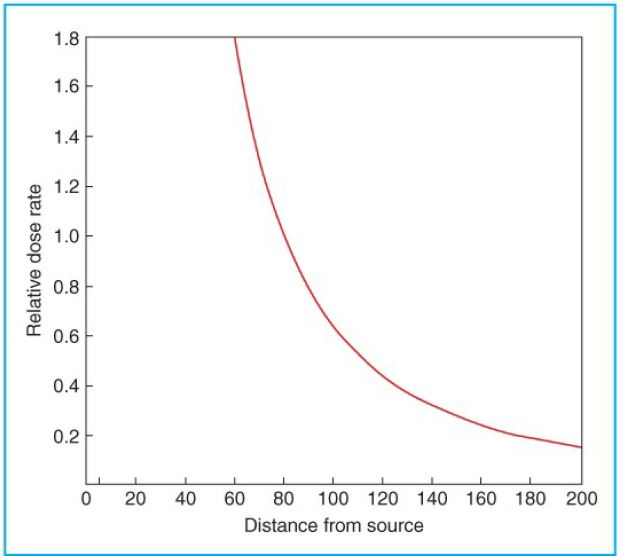
\includegraphics[width=0.4\textwidth]{Imagens/pdpSsd.JPG}
		\caption{Variação da PDP com a SSD}
		\label{fig:pdpSsd}
	\end{wrapfigure}

	A \textcolor{MediumOrchid}{\textbf{\textit{distância da fonte a superfície}}} em feixes clínicos é grande o suficiente para aproximar uma fonte com tamanho finito para uma fonte pontual, de modo que a \textcolor{MediumOrchid}{\textbf{\textit{fluência de fótons}}}, e portanto a taxa de dose no ar livre (taxa de exposição), irá variar com o IQD. 

	A \textcolor{MediumOrchid}{\textbf{\textit{PDP aumenta com a SSD como um resultado da IQD}}}. Embora a taxa de dose no ponto diminua com o aumento da SSD, a \textcolor{MediumOrchid}{\textbf{\textit{PDP é uma medida de dose relativa}}}, com respeito à dose na profundidade de referência, e portanto irá aumentar com o aumento da SSD. A \ref{fig:pdpSsd} mostra que a \textcolor{MediumOrchid}{\textbf{\textit{queda na taxa de dose entre dois pontos é muito maior em pequenas distâncias a partir da fonte do que para grandes distâncias à fonte}}}; Isso mostra que a PDP diminui mais rapidamente para menores SSDs do que para maiores SSDs. 

	Portanto, na rotina clínica a SSD deve ser estabelecida de modo que não diminua muito a taxa de dose, mas que seja grande o suficiente para aumentar a PDP em relação a $d_{max}$. Porém, existem tratamentos que requerem uma SSD estendida para conseguir um maior tamanho de campo, de modo que a PDP para a SSD padrão (80 cm por \ce{^{60}Co} e 100 cm para linacs) deve ser convertida para a SSD estendida utilizada no tratamento. 

	O \textcolor{DarkTurquoise}{\textbf{\textit{Fator Mayneord (F)}}} é um fator de correção menos preciso que considera apenas a IQD sem levar em consideração as mudanças no espalhamento devido ao aumento da SSD.

	\begin{figure}[h]
		\centering
		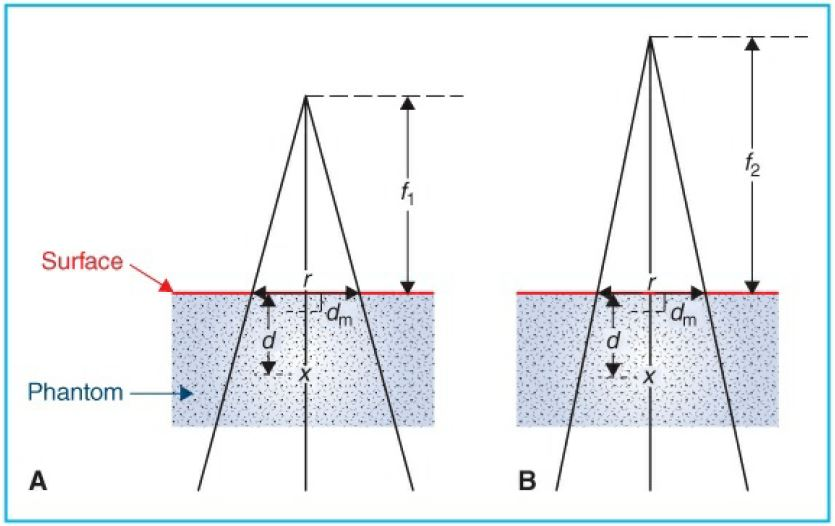
\includegraphics[width=0.7\textwidth]{Imagens/fatorF.JPG}
		\caption{Esquema para determinação do Fator F}
		\label{fig:fatorF}
	\end{figure}
	
	A \ref{fig:fatorF} mostra duas condições de irradiação variando a SSD, onde a $PDP(d,r,f)$ é a PDP na profundidade $d$ para uma $SSD = f$ e um tamanho de campo de lado $r$ (quadrado); Como a dose na profundidade é governada por 3 fatores: IQD, atenuação exponencial e pelo espalhamento; a PDP  para a $SSD = f_1$ é dada por:
	
		\begin{equation}
			PDP(d, r, f_1) = 100 \cdot \left(\frac{f_1 + d_{max}}{f_1 + d}\right)^2 \cdot e^{-\mu (d - d_{max})} \cdot K_s
			\label{eq:pdpParaSSD1}
		\end{equation}
	
	\begin{exemplo}[onde:]
		\begin{itemize}
			\item \textcolor{DarkTurquoise}{$\mathbf{\mu}$} é o coeficiente de atenuação linear efetivo para o feixe primário; e
			\item \textcolor{DarkTurquoise}{$\mathbf{K_s}$} é uma função que considera as mudanças na dose espalhada;
		\end{itemize}
	\end{exemplo}

	Considerando que $K_s$ não varia com a mudança da SSD, a PDP para a $SSD = f_2$ é dada por:

	\begin{equation}
		PDP(d, r, f_2) = 100 \cdot \left(\frac{f_2 + d_{max}}{f_2 + d}\right)^2 \cdot e^{-\mu (d - d_{max})} \cdot K_s
		\label{eq:pdpParaSSD2}
	\end{equation}

	Dividindo \ref{eq:pdpParaSSD2} pela \ref{eq:pdpParaSSD1}, temos que:

	\begin{equation}
		\frac{PDP(d, r, f_2)}{PDP(d, r, f_1)} = \left(\frac{f_2 + d_{max}}{f_1 + d_{max}}\right)^2 \cdot \left(\frac{f_1 + d}{f_2 + d}\right)^2
		\label{eq:razaoPDPF}
	\end{equation}

	Através da \ref{eq:razaoPDPF}, temos que:

		$$PDP(d, r, f_2) = F PDP(d, r, f_1)$$

	\begin{exemplo}[onde o Fator Mayneord:]
		\begin{equation}
			F = \left(\frac{f_2 + d_{max}}{f_1 + d_{max}}\right)^2 \cdot \left(\frac{f_1 + d}{f_2 + d}\right)^2
			\label{eq:fatorF}
		\end{equation}
	\end{exemplo}


	Isso mostra que o fator \textcolor{MediumOrchid}{\textbf{\textit{F é maior que 1 para $f_2 > f_1$ e menor que 1 quando $f_2 < f_1$}}}, o que reforça que a PDP aumenta com o aumento da SSD. Além disto, o fator F funciona bem para \textcolor{MediumOrchid}{\textbf{\textit{pequenos tamanhos}}} de campo devido à contribuição mínima da radiação espalhada para estes casos e, consequentemente, pode levar a grandes erros para condições extremas como feixe de baixa energias, campos largos, grandes profundidades e grandes mudanças na SSD pelo mesmo motivo (contribuição da radiação espalhada). 

	Para \textcolor{MediumOrchid}{\textbf{\textit{campos largos}}} e \textcolor{MediumOrchid}{\textbf{\textit{feixes de baixa energia}}} uma correção mais precisa é dada por:

		\begin{equation}
			F_{corr} = \frac{(1 + F)}{2}
		\end{equation}

\section{Razão Tecido-Ar (TAR)}

	Foi implementado para atender aos tratamentos em arco, onde a \textcolor{MediumOrchid}{\textbf{\textit{SSD varia com a posição do gantry}}}, porém a \textcolor{MediumOrchid}{\textbf{\textit{SAD (distância fonte eixo - isocentro) se mantém a mesma}}}, eliminando então às correções na PDP devido às variações na SSD. Portanto a TAR foi definida para \textcolor{MediumOrchid}{\textbf{\textit{eliminar a dependência com a SSD}}}. 

	\begin{figure}[h]
		\centering
		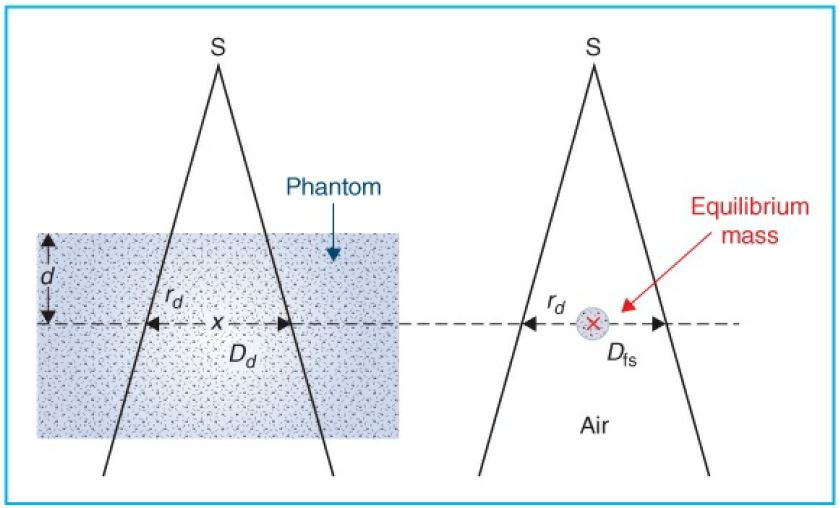
\includegraphics[width=0.7\textwidth]{Imagens/esquemaTAR.JPG}
		\caption{Esquema Para a Determinação do fator TAR}
		\label{fig:esquemaTAR}
	\end{figure}

	A TAR é definida como a \textcolor{MediumOrchid}{\textbf{\textit{razão entre a dose em um dado ponto no phantom $D_d$ e a dose no ar livre no mesmo ponto $D_{ar}$}}}, como mostra a \ref{fig:esquemaTAR}. Para uma determinada qualidade de feixe, a TAR depende apenas do \textcolor{MediumOrchid}{\textbf{\textit{tamanho de campo na profundidade $r_d$ e da profundidade $d$}}}, ou seja:

		\begin{equation}
			TAR(d, r_d) = \frac{D_d}{D_{ar}}
		\end{equation}


	\subsubsection*{Efeito da Distância}

	\textcolor{MediumOrchid}{\textbf{\textit{A TAR é independente da distância até a fonte uma vez que ela é dada pela razão entre duas doses medidas no mesmo ponto}}}, de modo que a dependência com a fluência de fótons é removida. Portanto, a TAR representa \textcolor{MediumOrchid}{\textbf{\textit{as mudanças na dose no ponto devido a apenas o espalhamento e a atenuação naquele ponto}}} no phantom quando comparado à dose obtida em  miniphantom colocado no mesmo ponto no ar livre. Portanto, A componente da TAR devido à \textcolor{MediumOrchid}{\textbf{\textit{atenuação}}} depende principalmente da \textcolor{MediumOrchid}{\textbf{\textit{profundidade}}}, uma vez que a atenuação varia exponencialmente com a profundidade. Já a componente do \textcolor{MediumOrchid}{\textbf{\textit{espalhamento}}}, é quase independente da divergência do feixe, dependendo apenas da \textcolor{MediumOrchid}{\textbf{\textit{profundidade e do tamanho do campo}}} naquela profundidade.

	\subsubsection*{Variação com a Energia, Profundidade e Tamanho de Campo}

	Para \textcolor{MediumOrchid}{\textbf{\textit{feixes de Megavoltagem}}}, a TAR \textcolor{MediumOrchid}{\textbf{\textit{aumenta}}} até um \textcolor{MediumOrchid}{\textbf{\textit{máximo}}} na profundidade de dose máxima \textcolor{MediumOrchid}{\textbf{\textit{$d_{max}$}}} e então \textcolor{MediumOrchid}{\textbf{\textit{diminui com a profundidade}}} aproximadamente exponencialmente. Para um feixe estreito (0 cm x 0 cm) onde a componente do espalhamento é aproximadamente nula, a TAR além de $d_{max}$ é aproximadamente:
	
		\begin{equation}
			TAR(d, 0) = e^{-\bar{\mu} (d - d_{max})}
		\end{equation}

	A medida que o tamanho de campo cresce, A TAR se torna mais complexa devido aos fótons espalhados, porém, a medida que a energia aumenta, os fótons são preferencialmente espalhados na direção de propagação do feixe primário e a TAR continua variando aproximadamente com a atenuação exponencial, através do coeficiente de atenuação efetivo para um determinado tamanho de campo.

	\subsection*{Fator de Retroespalhamento (BSF)}

	É também chamado de fator de espalhamento de pico (PSF); Este fator é dado pela \textcolor{MediumOrchid}{\textbf{\textit{TAR na profundidade de dose máxima}}}, ou seja:

		\begin{equation}
			BSF = \frac{D_{max}}{D_{ar}}
		\end{equation}

		\begin{equation}
			BSF = TAR(d_{max}, r_{d_{max}})
		\end{equation}

	\begin{exemplo}[onde:]
		\begin{itemize}
			\item \textcolor{DarkTurquoise}{$\mathbf{d_{max}}$} é a profundidade de dose máxima; e
			\item \textcolor{DarkTurquoise}{$\mathbf{r_{d_{max}}}$} é o tamanho de campo projetado em $d_{max}$.
		\end{itemize}
	\end{exemplo}
	
	Assim como o fator TAR, o \textcolor{MediumOrchid}{\textbf{\textit{BSF é independente da SSD}}} e depende apenas da \textcolor{MediumOrchid}{\textbf{\textit{qualidade do feixe e do tamanho de campo}}}. O fator BSF é muito maior para feixes de KV comparado com feixes de MV para um mesmo tamanho de campo. A \ref{fig:bsf} mostra a diferença do BSF para diferentes qualidades de feixes e diferentes tamanhos de feixe. 

	\begin{figure}[h]
		\centering
		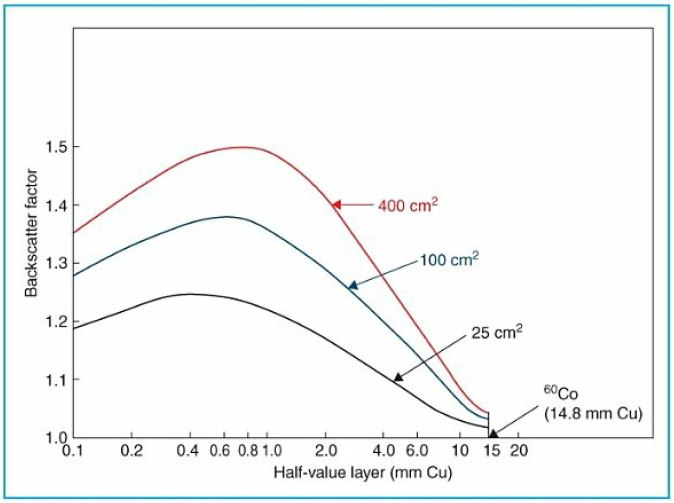
\includegraphics[width=0.8\textwidth]{Imagens/bsf.JPG}
		\caption{BSF para diferentes qualidades de feixe e diferentes tamanhos de campo}
		\label{fig:bsf}                
	\end{figure}

	Por exemplo, o BSF para o \ce{^{60}Co} para um campo 10 cm x 10 cm é de 1.036, o que significa que a Dose máxima é 3.6\% maior no phantom que a dose no ar livre. Esse aumento é devido a contribuição da radiação espalhada nos tecidos acima e abaixo que alcança o ponto de $D_{m}$. A medida que a energia aumenta, o BSF é reduzido até que, em energias acima de 8 MV, a componente devido a radiação espalhada que alcança $d_{max}$ se torna mínima e o fator BSF se aproxima do seu valor mínimo, igual a 1. 


	\subsection*{Relação entre a PDP e a TAR}

	\begin{figure}[h]
		\centering
		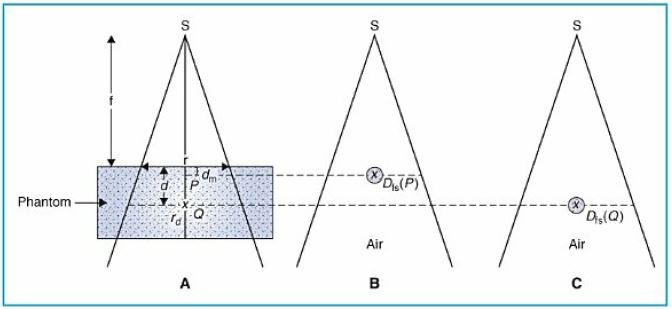
\includegraphics[width=0.8\textwidth]{Imagens/pdpETar.JPG}
		\caption{Relação entre a PDP e a TAR}
		\label{fig:pdpETar}                
	\end{figure}

	A PDP e a TAR podem ser relacionadas, como mostra a \ref{fig:pdpETar}. Sendo a $TAR(d, r_d)$ a TAR no ponto Q para um tamanho de campo $r_d$ na profundidade $d$; E seja $r$ o tamanho de campo na superfície, $f$ a SSD e $d_{max}$ a profundidade de referência igual a profundidade de dose máxima no ponto P. Seja $D_{fs}(P)$ a dose no ar livre no ponto P e $D_{fs}(Q)$ a dose no ar livre no ponto Q; A dose em $D_{fs}(P)$ e $D_{fs}(Q)$ estão relacionadas através da IQD da seguinte forma:

		\begin{equation}
			\frac{D_{fs}(Q)}{D_{fs}(P)} = \left(\frac{f + d_{max}}{f + d}\right)^2
		\end{equation}

	Os tamanhos de campo $r$ e $r_d$ estão relacionados através da seguinte equação:

		\begin{equation}
			r_d = r \cdot \frac{f + d}{f}
		\end{equation}

	Pela definição de TAR, temos que:

		$$TAR(d, r_d) = \frac{D_d(Q)}{D_{fs}(Q)}$$

	\begin{equation}
		D_d{Q} = TAR(d, r_d) \cdot D_{fs}(Q)
	\end{equation}

	Dado que 

		$$BSF(r) = \frac{D_{max}(P)}{D_{fs}(P)}$$

		$$D_{max}{P} = D_{fs}(P) \cdot BSF(r)$$

	E pela definição, a $PDP(d, r, f)$ é dada por:

		$$PDP(d, r, f) = \frac{D_d(Q)}{D_{max}(P)} \cdot 100$$

	Temos que:

		$$PDP(d, r, f) = TAR(d, r_d) \cdot \frac{1}{BSF(r)} \cdot \frac{D_{fs}(Q)}{D_{fs}(P)} \cdot 100$$

	Chegando então na seguinte relação:

	\begin{equation}
		PDP(d, r, f) = TAR(d, r_d) \cdot \frac{1}{BSF(r)} \cdot \left(\frac{f + d_{max}}{f + d}\right)^2 \cdot 100
		\label{eq:tarParaPdp}
	\end{equation}

	\subsection*{Método TAR para corrigir a PDP para diferentes SSDs}

	Este é um método mais preciso que o Fator F Mayneord pois a TAR considera o espalhamento e está relacionada com a PDP a partir da \ref{eq:tarParaPdp}.

	Supondo que $f_1$ é a SSD para o qual a PDP foi determinada e $f_2$ é a SSD alterada, para o qual deseja-se obter a nova PDP. Seja $r$ o tamanho de campo na superfície e $d$ a profundidade em ambos os casos. Com base na \ref{fig:fatorF}, seja $r_{d, f_1}$ e $r_{d, f_2}$ os tamanhos de campo projetados na profundidade $d$ para a as SSDs $f_1$ e $f_2$, de modo que:

		$$r_{d, f_1} = r \cdot \frac{f_1 + d}{f_1}$$

		$$r_{d, f_2} = r \cdot \frac{f_2 + d}{f_2}$$

	A partir da \ref{eq:tarParaPdp} temos que:

		$$PDP(d, r, f_1) = TAR(d, r_{d, f_1}) \cdot \frac{1}{BSF(r)} \cdot \left(\frac{f_1 + d_{max}}{f_1 + d}\right)^2 \cdot 100$$

	e 

		$$PDP(d, r, f_2) = TAR(d, r_{d, f_2}) \cdot \frac{1}{BSF(r)} \cdot \left(\frac{f_2 + d_{max}}{f_2 + d}\right)^2 \cdot 100$$


	Dividindo $PDP(d, r, f_2)$ por $PDP(d, r, f_1)$ temos que:

	\begin{equation}
		\frac{PDP(d, r, f_2)}{PDP(d, r, f_1)} = \frac{TAR(d, r_{d, f_2})}{TAR(d, r_{d, f_1})} \cdot \left[\left(\frac{f_2 + d_{max}}{f_1 + d_{max}}\right)^2 \cdot \left(\frac{f_1 + d}{f_2 + d}\right)^2\right]
		\label{eq:metodoTar}
	\end{equation}

	Onde 

	$$\left(\frac{f_2 + d_{max}}{f_1 + d_{max}}\right)^2 \cdot \left(\frac{f_1 + d}{f_2 + d}\right)^2 = F = Fator \; Mayneord$$

	Portanto, o Método da TAR corrige o fator F pela razão das TARs para os tamanhos de campo projetados na profundidade d para diferentes SSDs. Outra equação, desenvolvida por Burns é utilizada para converter a PDP de uma SSD para outra:

	\begin{equation}
		PDP(d, r, f_2) = PDP(d, \frac{r}{\sqrt{F}}, f_1) \cdot \frac{BSF(r/\sqrt{F})}{BSF(r)} \cdot F
		\label{eq:burns}
	\end{equation}

	A \ref{eq:burns} se baseia no fato de que as TARs são independentes da distância até a fonte. Esta equação pode ser utilizada naqueles casos onde a TAR não está disponível mas a PDP é determinada para um valor padrão de SSD juntamente com os valores de BSF para vários tamanhos de campo. 

	Para feixes com energias superiores a 8 MV, a variação da PDP com o tamanho de campo é muito pequena de modo que o retroespalhamento pode ser negligenciado e tanto a  \ref{eq:metodoTar} quanto a \ref{eq:burns} podem ser aproximadas para o fator Mayneord.

	\subsection*{Cálculo de Dose em Terapia com Arco}

	O cálculo de dose na profundidade com terapias em arco envolve a determinação da TAR média no isocentro. O contorno do paciente é delineado em um plano contendo o eixo de rotação e o isocentro é então colocado dentro do contorno, normalmente no centro do tumor ou a poucos centímetros dele. O raio é então desenhado a partir desse ponto em intervalos de ângulos, (\ang{20}) como mostra a \ref{fig:tarArco}. 

	\begin{figure}[h]
		\centering
		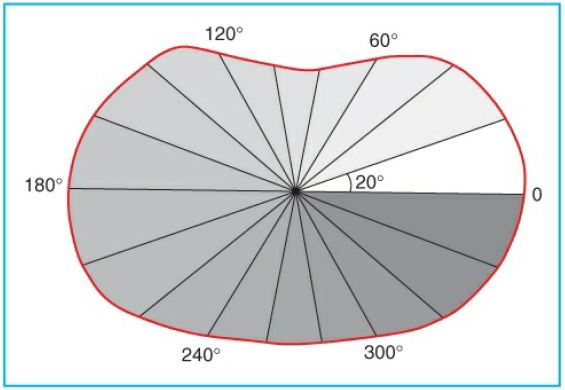
\includegraphics[width=0.8\textwidth]{Imagens/tarArco.JPG}
		\caption{Contorno para determinar a TAR média}
		\label{fig:tarArco}                
	\end{figure}

	Cada raio representa a profundidade para o qual a TAR será determinada a partir de uma tabela de TAR, para uma dada energia de feixe e tamanho de campo definido no isocentro. A TAR é somada e a média é determinada como mostra a \ref{fig:tabelaTarArco}.


	\begin{figure}[h]
		\centering
		\fcolorbox{DarkTurquoise}{white}{%
		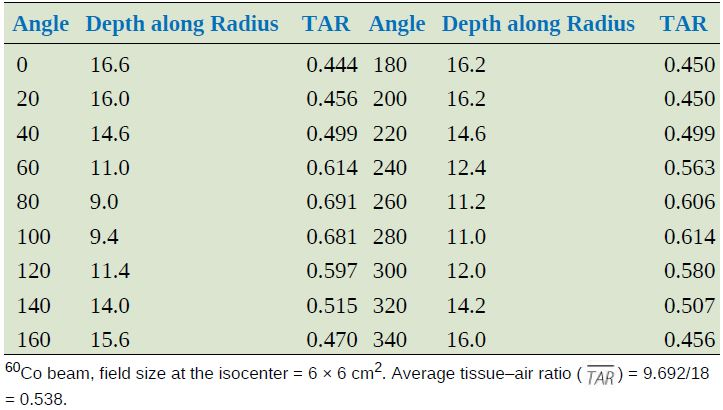
\includegraphics[width=0.8\textwidth]{Imagens/tabelaTarArco.JPG}
		}%
		\caption{Determinação da TAR média no centro de rotação}
		\label{fig:tabelaTarArco}
	  \end{figure}


	\section{Razão Espalhamento-Ar (SAR)}

	A SAR é definida para calcular a dose espalhada no meio, devido a necessidade de se determinar separadamente o feixe primário da radiação espalhada na dosimetria de campos irregulares.

	A SAR pode ser definida como a razão entre a dose espalhada em um dado ponto no phantom e a dose no mesmo ponto porém no ar livre. A SAR é independente da SSD mas depende da energia do feixe, profundidade e tamanho de campo. 

	Como a dose espalhada em um ponto é igual a dose total menos a dose devido ao feixe primário nesse ponto, a SAR pode ser definida como:

		\begin{equation}
			SAR(d,r_d) = TAR(d,r_d) - TAR(d, 0)
		\end{equation}

		\begin{exemplo}[onde:]
			\begin{itemize}
				\item \textcolor{CarnationPink}{$\mathbf{TAR(d,r_d)}$} determina a dose total na profundidade $d$ para o tamanho de campo $r_d$; 
				\item \textcolor{CarnationPink}{$\mathbf{TAR(d, 0)}$} determina a componente devido a apenas o feixe primário (campo estreito)
			\end{itemize}
		\end{exemplo}

	Como a SAR foi primeiramente definida para determinar o espalhamento para campos irregulares, os seus valores são tabulados como função da profundidade e do raio de um campo circular nessa profundidade. E como os dados da SAR são derivados a partir da TAR para campos quadrados ou retangulares, o raio do círculo equivalente pode ser obtido através da \ref{eq:raioEquivalente}.

	\subsection*{Método de Clarkson para Cálculo de Dose de Campos irregulares}
	
	Como a base de dados para os cálculos de dose são determinadas para campos quadrados é necessário utilizar métodos para corrigir esses fatores ao utilizar campos irregulares, como o manto utilizado para o tratamento de linfoma de Hodgkin. 

	O método de Clarkson se baseia no princípio de que a componente de espalhamento da dose na profundidade, que depende do tamanho e forma do campo, pode ser calculada separadamente a partir da componente primária, que é independente do tamanho e da forma do campo. 


	\begin{figure}[h]
		\centering
		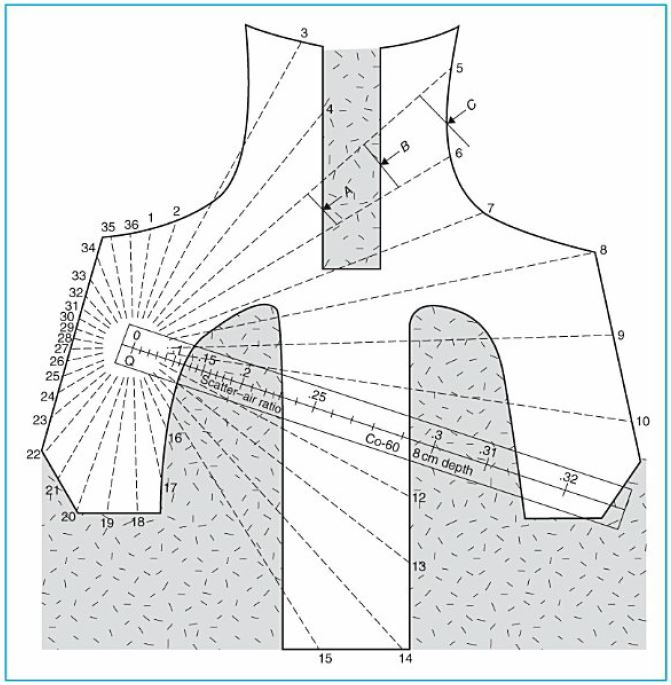
\includegraphics[width=0.8\textwidth]{Imagens/clarkson.JPG}
		\caption{Setores para método de Clarkson}
		\label{fig:clarkson}                
	\end{figure}

	Considerando um campo irregular, como mostra a \ref{fig:clarkson}, assumindo que a seção transversal do campo ocorre na profundidade $d$ e está perpendicular ao eixo do feixe. Seja $Q$ o ponto de cálculo no plano da seção transversal do feixe; Os raios são desenhados a partir de Q para dividir o campo em setores elementares. Cada setor é caracterizado pelo seu raio e pode ser considerado como uma parte de um campo circular de mesmo raio. Supondo que cada setor tenha um ângulo de \ang{10}, então a contribuição da componente de espalhamento para este setor será de \ang{10}/\ang{360} $=$ 1/36 da contribuição de um campo circular com o mesmo raio centrado em Q. Assim, a contrinuição do espalhamento de todos os setores pode ser calculada e somada considerando cada setor como sendo uma parte de seu próprio círculo cuja SAR é conhecida e tabelada. 

	A SAR média ($\bar{SAR}$) no ponto $Q$  pode ser então determinada considerando a soma de todos os valores de SAR para os setores, dividido pelo número total de setores. Para os setores que passam através de áreas bloqueadas, a SAR líquida é determinada subtraindo a contribuição do espalhamento da parte bloqueada do setor. Por Exemplo, $(SAR)_{QC_{liq}} = (SAR)_{QC} - (SAR)_{QB} + (SAR)_{QA}$. A $\bar{SAR}$ calculada é convertida para a $\bar{TAR}$ através da equação:

		\begin{equation}
			\bar{TAR} = TAR(0) + \bar{SAR}
		\end{equation}

	onde a $TAR(0)$ é a razão tecido-ar para o campo 0 x 0, dada por:

		$$TAR(0) = e^{-\bar{\mu} (d - d_{max})}$$

	\begin{exemplo}[onde:]
		\begin{itemize}
			\item \textcolor{DarkTurquoise}{$\mathbf{\bar{\mu}}$} é o coeficiente de atenuação linear médio;
			\item \textcolor{DarkTurquoise}{$\mathbf{d}$} é a profundidade do ponto Q.
		\end{itemize}
	\end{exemplo}

	A PDP ($\%DD$) no ponto $Q$ pode ser calculada com relação a $D_{max}$ no eixo central através da \ref{eq:tarParaPdp}:

		\begin{equation}
			\%DD = 100 \times \bar{TAR} \times \left(\frac{f + d_{max}}{f + d}\right)^2 \frac{1}{BSF}
		\end{equation}

	\begin{exemplo}[onde:]
		\begin{itemize}
			\item \textcolor{DarkTurquoise}{$\mathbf{BSF}$} é o fator de retroespalhamento que pode ser calculado através do método de Clarkson, onde envolve a TAR na profundidade de dose máxima $d_{max}$ no eixo central, utilizando o contorno do campo ou raio projetado na profundidade de $d_{max}$.
		\end{itemize}
	\end{exemplo}

\section{Algoritmos Baseados em Modelo}

	Os algoritmos baseados em modelos para o cálculo de distribuições de dose em um paciente podem ser categorizados em três tipos principais:

	\begin{itemize}
		\item \textcolor{DarkTurquoise}{\textbf{Cálculo analítico simples:}}
		
		O método de cálculo analítico simples é uma abordagem relativamente básica que se baseia no cálculo analítico do espalhamento de Compton de primeira ordem. Nesse método, a dose primária no ponto de interesse é complementada pela contribuição do espalhamento. No entanto, essa técnica faz a suposição de um feixe paralelo de fótons com uma única energia e não leva em consideração o espalhamento de ordem superior nem as heterogeneidades presentes no paciente.
		 
		\item \textcolor{DarkTurquoise}{\textbf{Método de convolução-sobreposição:}} 
		
		O método de convolução-sobreposição leva em consideração a natureza indireta da deposição de dose resultante das interações de fótons com o tecido. Esse método separa as interações primárias de fótons do transporte de fótons espalhados e partículas carregadas geradas por meio do efeito fotoelétrico, espalhamento de Compton e produção de pares.


		\item \textcolor{DarkTurquoise}{\textbf{Método de Monte Carlo:}}
		
		O método de Monte Carlo é considerado o mais promissor para o cálculo de dose baseado em modelo. Ele utiliza distribuições de probabilidade bem estabelecidas para simular as interações de fótons e elétrons com o paciente e o transporte dessas partículas dentro do paciente. Os métodos de Monte Carlo são essenciais para caracterizar o feixe clínico e também podem calcular diretamente distribuições de dose de fótons para um paciente específico e sua geometria de tratamento. No entanto, a principal limitação dos cálculos diretos de Monte Carlo é o tempo significativo necessário para calcular um grande número de histórias a fim de reduzir as incertezas estocásticas. No entanto, espera-se que avanços na tecnologia de computadores reduzam os tempos de cálculo de Monte Carlo, tornando-o o método padrão no planejamento de tratamento radioterápico. Para realizar cálculos de distribuição de dose baseados em Monte Carlo, são obtidas as densidades eletrônicas dos diferentes tecidos dentro de pacientes individuais, usando tomógrafos computadorizados (TC) ou simuladores de TC, que são componentes cruciais do processo de cálculo.
	\end{itemize}

\section{Medidas Relativas Para Caracterização do Feixe com Câmaras de Ionização}
	
\begin{exemplo}[Aplicações em Cada Medida:]
	\begin{itemize}
		\item \textcolor{DarkTurquoise}{\textbf{Câmaras de ionização cilíndricas de volume relativamente grande (0.6 cc):}} são utilizadas para medir doses e taxas de dose em pontos de referência em um fantoma para feixes de fótons de megavoltagem e feixes de elétrons acima de 10 MeV para garantir um sinal razoável e uma boa relação sinal-ruído.

		\item \textcolor{DarkTurquoise}{\textbf{câmaras de ionização de pequeno volume (0.1 cc)}} são utilizadas para medidas de distribuições relativas de dose, como curvas PDD e perfis de feixe, para feixes de fótons além da profundidade de dose máxima ($d_{max}$) e para feixes de elétrons, pois fornecem alta resolução espacial.
		
		\item \textcolor{DarkTurquoise}{\textbf{Câmaras de ionização de placas paralelas:}} são utilizadas para medições de doses superficiais e doses na região de buildup para feixes de fótons. Essas câmaras são equipadas com uma fina janela de eletrodo polarizador para capturar a dose superficial e possuem um pequeno espaçamento entre eletrodos (tipicamente 1 mm) para melhor resolução espacial.
		
		\item As polaridades positiva e negativa de uma câmara de ionização de placas paralelas são usadas para medir uma curva típica de PDD para feixes de fótons de megavoltagem na região de buildup e além. A diferença nos sinais entre as duas polaridades é mais significativa na superfície do fantoma e diminui com a profundidade até desaparecer em $d_{max}$ e além. Na região de buildup, uma câmara de ionização cilíndrica apresentará leituras artificialmente altas devido à sua espessura excessiva da parede, enquanto uma câmara de placas paralelas fornece medições precisas.
		
		\item  Na região de buildup, são medidas as polaridades positiva e negativa de uma câmara de ionização de placas paralelas, e a leitura média entre as duas polaridades é considerada o valor real de dose. Essa média compensa a corrente Compton gerada pelas interações de fótons no eletrodo de medição, que causa um aumento na leitura para a polaridade positiva e uma diminuição na leitura para a polaridade negativa.
		
		\item Para profundidades além de  $d_{max}$, ambas as polaridades da câmara fornecem a mesma leitura porque o equilíbrio eletrônico é alcançado no eletrodo de medição.
		
		\item  A eficiência de coleta iônica em uma câmara de ionização depende não apenas da diferença de potencial entre os eletrodos polarizante e de medição, mas também da taxa de dose dentro da câmara. Ao medir doses relativas na profundidade, as alterações na recombição iônica com a profundidade são geralmente ignoradas, pois a perda de recombição iônica em câmaras de bom desempenho geralmente é de 2\% ou menos.
		
		\item \textcolor{DarkTurquoise}{\textbf{}} As razões de poder freamento (água para ar) e os fatores de correção da câmara são dependentes da profundidade, e seu impacto deve ser considerado com base na situação específica e na precisão desejada ao medir doses em profundidade com câmaras de ionização. Em feixes de fótons, a razão de poder de freamento restrita de água para ar é essencialmente independente da profundidade além de $d_{max}$. Em feixes de elétrons, a razão de poder de freamento restrito de água para ar varia significativamente com a profundidade, exigindo correções na curva de ionização medida ao determinar a dose relativa.
		
		\item Para câmaras não blindadas, como câmaras tipo Farmer, o fator de correção de perturbação de fluência também varia com a energia em profundidade em feixes de elétrons. Portanto, câmaras de ionização de placas paralelas bem blindadas são mais adequadas para medir doses relativas em feixes de elétrons em comparação com câmaras do tipo "thimble".
	\end{itemize}
\end{exemplo}


\pagebreak
\bibliography{ref.bib}
\end{document}